\section{Конструкторский раздел}

% NOTE:
% В конструкторском разделе описывается разрабатываемый метод
% В случае если в бакалаврском проекте разрабатывается новый метод или алгоритм, необходимо подробно изложить их суть, привести все необходимые для их реализации математические выкладки, обосновать последовательность этапов выполнения
% При этом для каждого этапа следует выделить необходимые исходные данные и получаемые результаты
% Для описания метода или алгоритма - Схема алгоритма
% В конце описания разработанного алгоритма должны быть приведены выбранные способы тестирования и сами тесты
% Перед формированием тестовых наборов данных целесообразно указать выделенные классы эквивалентности
% (тут же могут быть приведены выкладки по теоретическим рассчетам требуемой памяти и эффективности алгоритма; эти результаты могут быть использованы для обоснования правильности выбора метода из уже имеющихся альтернативных вариантов)
% Также должно быть приведено описание структуры разрабатываемого ПО, оно включает в себя:
% - описание общей структуры - определение основных частей (компонентов) и их взаимосвязей по управлению и по данным
% - декомпозицию компонентов и построение структурных иерархий
% - проектирование компонентов
% Для графического представления такого описания (если есть необходимость), следует использовать IDEF0 с декомпозицией исходной задачи на несколько уровней

% Рек. Объем 25-30 страниц

\subsection{Требования и ограничения метода}

Метод выделения составных частей научного текста на основе анализа распределения пикселей в сканирующей строке должен:
\begin{enumerate}
    \item Работать с одноколоночными Манхэттенскими макетами документов;
    \item Выделять текстовые блоки;
    \item Выделять таблицы;
    \item Выделять листинги;
    \item Выделять схемы алгоритмов;
    \item Выделять рисунки;
    \item Выделять графики;
    \item Работать на основе простых правил и эвристик, без использования нейросетей.
\end{enumerate}

% Разработать метод выделения ... строке
% Изложить особенности предложенного метода

\subsection{Описание разрабатываемого метода}

Поставленная задача решается в четыре этапа:
\begin{enumerate}
    \item Преобразование PDF документа в изображения;
    \item Первичная разметка страниц;
    \item Создание уточненной разметки на основе первичной;
    \item Объединение уточненной разметку в более крупные блоки.
\end{enumerate}

Разметка, ее уточнение и объединение происходят на основе определенных правил, которые будут описаны в данном разделе далее.

Основные этапы разрабатываемого метода представлены на IDEF0 диаграмме первого уровня (см. Рисунок \ref{fig:a1}).

\begin{figure}[H]
	\centering
	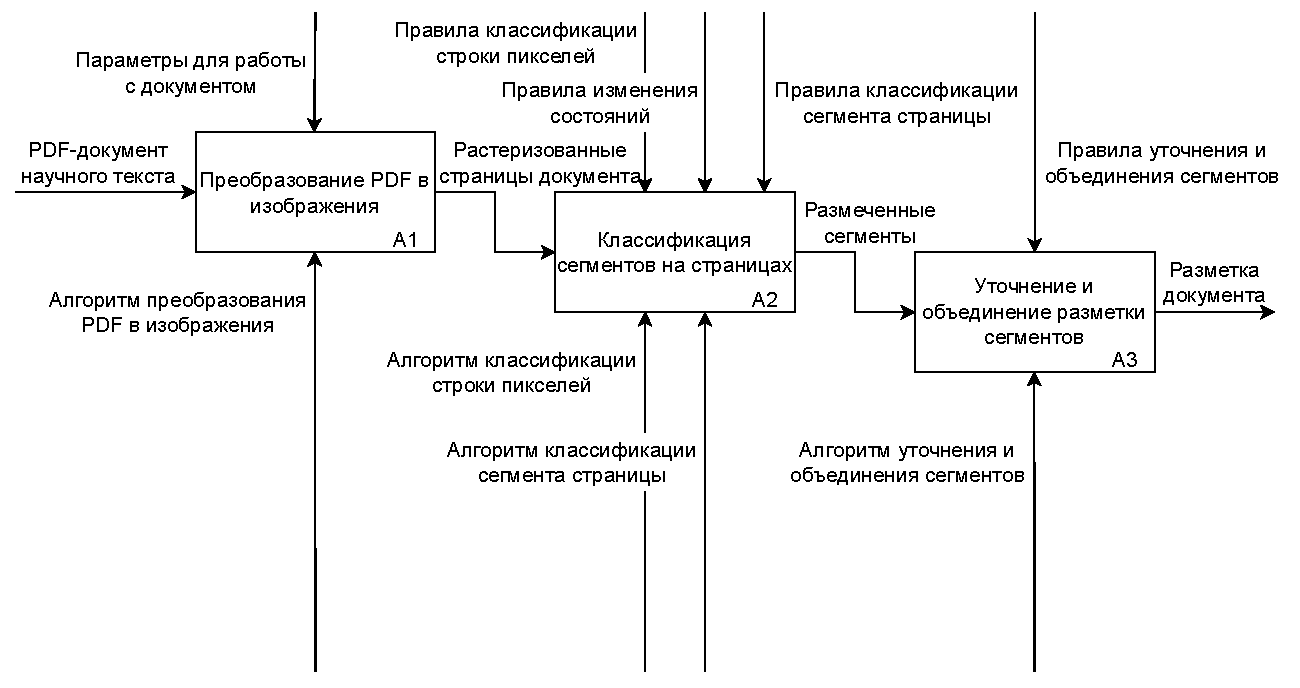
\includegraphics[width=\textwidth]{diag/a1-big.pdf}
	\caption{IDEF0-диаграмма метода выделения составных частей научного текста на основе анализа распределения пикселей в сканирующей строке}
	\label{fig:a1}
\end{figure}

\subsubsection{Первичная разметка}

Исходные данные --- изображение страницы документа.
Получаемый результат --- разметка страницы и информация о каждом сегменте на ней.

Разметка страницы --- массив кортежей типа
$$
(y\_start, y\_end, C),
$$
где $y\_start$ --- $y$-координата начала сегмента в пространстве изображения, $y\_end$ --- $y$-координата конца сегмента в пространстве изображения, $C$ --- класс сегмента, где $C \subseteq$ $\{$Фон, Немного текста, Много текста, Цвет, Черная линия средней длины, Длинная черная линия, Не определено$\}$.

Такое множество классов было выделено по двум причинам.
Во-первых, на основе распределения пикселей в строке ее уже можно причислить к одному из перечисленных классов.
Во-вторых, на основе принадлежности строки к одному из классов можно делать предположения насчет класса сегмента, которому строка принадлежит.

Так, если строка классифицируется как <<Много текста>> можно предположить, что сегмент вероятно принадлежит классу <<Текст>>.

Если строка классифицируется как <<Цвет>>, можно предположить, что сегмент вероятно принадлежит классу <<Рисунок>> или <<График>>.

Если строка классифицируется как <<Черная линия средней длины>>, можно предположить, что сегмент вероятно принадлежит классу <<Схема алгоритма>>.

Если строка классифицируется как <<Длинная черная линия>>, можно предположить, что сегмент вероятно принадлежит классу <<Таблица>> или <<Листинг>>.

Информация о сегменте содержит следующие данные:
\begin{enumerate}
    \item start --- ордината начала сегмента;
    \item end --- ордината конца сегмента;
    \item count\_long\_black\_line --- количество раз, когда при разметке сегмента встретилась строка, идентифицированная, как <<Длинная черная линия>>;
    \item count\_single\_long\_black\_line --- количество раз, когда при разметке сегмента встретилась строка, идентифицированная, как <<Длинная черная линия>>, считая несколько подряд идущих <<Длинных черных линий>> за одну;
    \item count\_medium\_black\_line --- количество раз, когда при разметке сегмента встретилась строка, идентифицированная, как <<Черная линия средней длины>>;
    \item count\_single\_medium\_black\_line --- количество раз, когда при разметке сегмента встретилась строка, идентифицированная, как <<Черная линия средней длины>>, считая несколько подряд идущих <<Черных линий средней длины>> за одну;
    \item count\_total\_medium\_black\_line --- количество раз, когда при разметке сегмента встретилась строка, идентифицированная, как <<Черная линия средней длины>>, с учетом всех <<Черных линий черной длины>> если таких было зафиксировано несколько внутри одной сканирующей строки;
    \item count\_many\_text --- количество раз, когда при разметке сегмента встретилась строка, идентифицированная, как <<Много текста>>;
    \item count\_few\_text --- количество раз, когда при разметке сегмента встретилась строка, идентифицированная, как <<Немного текста>>;
    \item count\_color --- количество раз, когда при разметке сегмента встретилась строка, идентифицированная, как <<Цвет>>;
    \item count\_undefined --- количество раз, когда при разметке сегмента встретилась строка, идентифицированная, как <<Не определено>>;
    \item count\_white\_px --- количество белых пикселей в сегменте;
    \item count\_color\_px --- количество цветных пикселей в сегменте;
    \item count\_gray\_px --- количество черных пикселей в сегменте (сумма трех данных счетчиков дает общее количество пикселей в сегменте);
    \item heatmap\_black --- массив, $i$-й элемент которого отражает количество черных пикселей в $i$-й колонке пикселей сегмента;
    \item heatmap\_color --- массив, $i$-й элемент которого отражает количество цветных пикселей в $i$-й колонке пикселей сегмента.
\end{enumerate}

Данная информация будет использоваться для уточнения разметки в следующем этапе.

Первичная разметка создается в результате классификации строк на основе распределения пикселей в них и изменения состояний конечного автомата первичной разметки.

Диаграмма изменения состояний конечного автомата изображена на рисунке \ref{fig:fsm-full}.
Классификация любого сегмента начинается из состояния <<Фон>>, и заканчивается в состоянии <<Фон>>, причем в результате классификации сегменту присваивается класс в соответствии с предпоследним состоянием, в котором находился конечный автомат (до последнего <<Фона>>).

\begin{figure}[H]
	\centering
	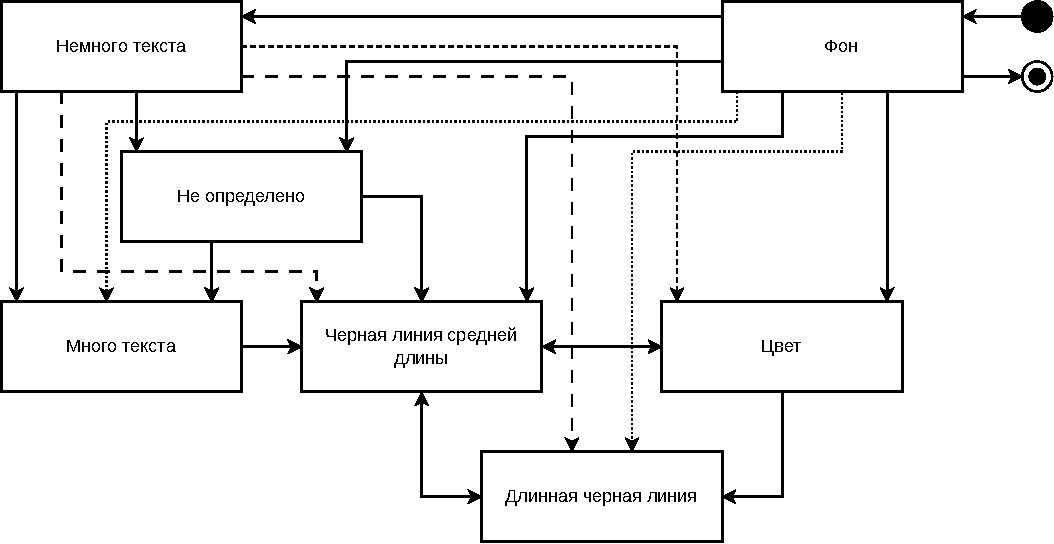
\includegraphics[width=\textwidth]{diag/fsm.full.pdf}
	\caption{Конечный автомат, все состояния}
	\label{fig:fsm-full}
\end{figure}

Из состояния <<Фон>> можно попасть в любое состояние.
Из состояния <<Немного текста>> можно попасть в любое состояние, кроме <<Фона>>.
Поэтому на рисунке \ref{fig:fsm-slim} изображена редуцированная диаграмма конечного автомата, опускающая состояния <<Фон>> и <<Немного текста>>.

\begin{figure}[H]
	\centering
	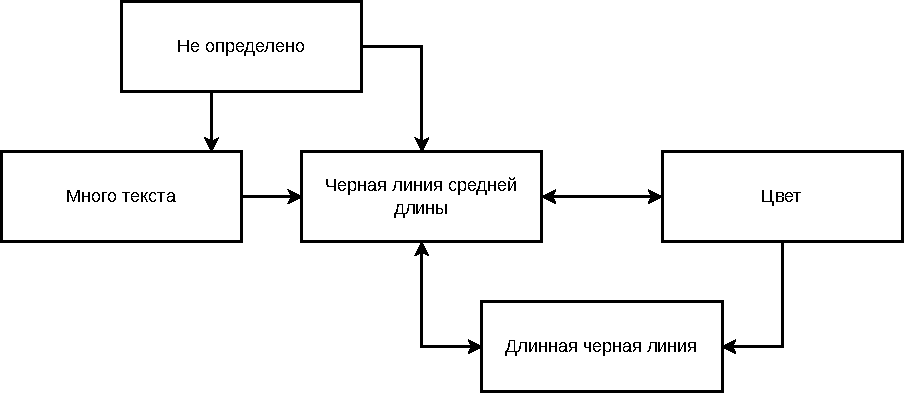
\includegraphics[width=\textwidth]{diag/fsm.slim.pdf}
	\caption{Конечный автомат, состояния кроме <<Немного текста>> и <<Фон>>}
	\label{fig:fsm-slim}
\end{figure}

На рисунке \ref{fig:primary-markup} ниже изображена схема алгоритма классификации конкретной сканирующей строки.

\begin{figure}[H]
	\centering
	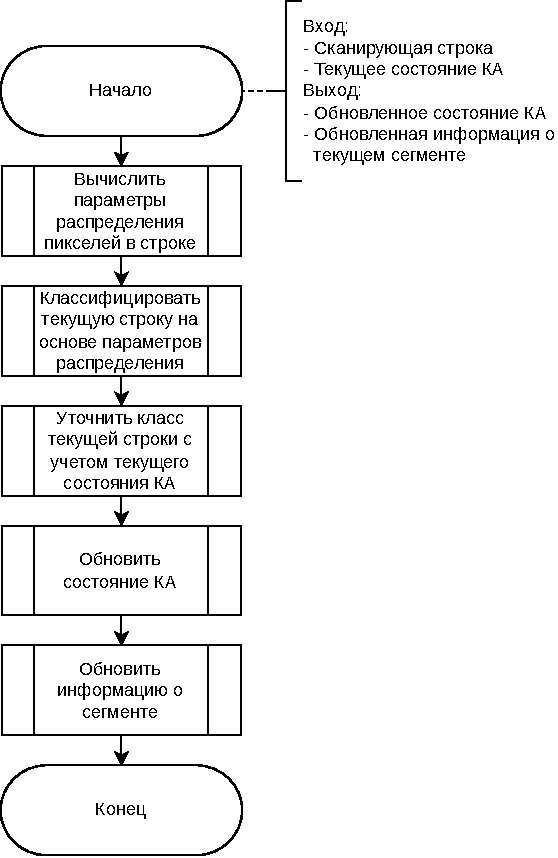
\includegraphics[width=0.7\textwidth]{diag/primary-markup.pdf}
	\caption{Разметка сканирующей строки}
	\label{fig:primary-markup}
\end{figure}

\subsubsection*{Классификация строки}

Классификация строки производится на основе следующих параметров распределения пикселей в ней:
\begin{enumerate}
    \item count\_white --- количество белых пикселей в строке;
    \item count\_color --- количество цветных пикселей в строке;
    \item count\_gray --- количество серых (почти черных) пикселей в строке;
    \item comp\_lengths --- массив длин участков подряд идущих не белых пикселей;
    \item gap\_lengths --- массив длин промежутков (белых пикселей) между участками подряд идущих не белых пикселей;
    \item gray\_comp\_lengths --- массив длин участков подряд идущих серых пикселей;
    \item color\_comp\_lengths --- массив длин участков подряд идущих цветных пикселей;
    \item first\_nonwhite\_index --- индекс первого не белого пикселя в строке.
\end{enumerate}

\subsubsection*{Классификация как <<Фон>>}

Строка классифицируется как <<Фон>>, если выполнено условие <<first-\_nonwhite\_index не установлен>> --- в строке не нашлось не белых пикселей.

\subsubsection*{Классификация как <<Длинная черная линия>>}

Строка классифицируется как <<Длинная черная линия>>, если: строка содержит единственную серую компоненту И эта компонента достаточно длинная.

Содержание единственной серой компоненты определяется на основе одновременного выполнения следующих условий:
\begin{itemize}
    \item Длина comp\_lengths равна 1;
    \item Длина gap\_lengths равна 0;
    \item Длина color\_comp\_lengths равна 0.
\end{itemize}

Длина серой компоненты для классификации строки как <<Длинная черная линия>> считается достаточно большой, если count\_gray больше некоторого параметра, который является произведением длины строки на некоторую наперед заданную константу, принимающую значения от 0 до 1, например 1/2.

\subsubsection*{Классификация как <<Черная линия средней длины>>}

Строка классифицируется как <<Черная линия средней длины>>, если строка содержит компоненту, длина которой больше некоторого параметра, который является произведением длины строки на некоторую наперед заданную константу, принимающую значения от 0 до 1, например, 1/16.

\subsubsection*{Классификация как <<Много текста>>}

Строка классифицируется как <<Много текста>>, если она либо содержит очень много черных компонент, либо содержит много черных компонент и не содержит цвета.

Считается, что строка содержит очень много черных компонент, если длина comp\_lengths превышает некоторую наперед заданную константу, например 100.

Считается, что строка содержит много черных компонент, если длина comp\_lengths превышает некоторую наперед заданную константу, например 80.

Таким образом, если строка содержит очень много черных компонент, она будет классифицирована как <<Много текста>> вне зависимости от наличия в ней цвета.

\subsubsection*{Классификация как <<Цвет>>}

Строка классифицируется как <<Цвет>>, если count\_color больше нуля.

\subsubsection*{Классификация как <<Немного текста>>}

Строка классифицируется как <<Немного текста>>, если содержит немного компонент И компоненты преимущественно небольшого размера И промежутки между компонентами преимущественно небольшого размера И отсутствуют большие промежутки.

Считается, что компоненты и/или промежутки между компонентами преимущественно небольшого размера, если среднее арифметическое comp-\_lengths и/или gap\_lengths меньше некоторой наперед заданной константы, например, 20 пикселей.

Считается, что большие промежутки отсутствуют, если в массиве gap\_lengths отсутствуют элементы с индексом стандартного отклонения больше шести.

Индекс стандартного отклонения $Z$ для элемента массива $x$ вычисляется по формуле:
$$
Z(x) = \frac{x - \mu}{\sigma},
$$
где $\mu$ --- среднее значение элементов массива, $\sigma$ --- стандартное отклонение элементов массива.

\subsubsection*{Классификация как <<Не определено>>}

В остальных случаях строка классифицируется как <<Не определено>>.

\subsubsection*{Изменение состояний КА}

Далее будут представлены таблицы переходов состояний конечного автомата, в которых некоторые правила были подобраны исходя из логических соображений, а некоторые --- эмпирическим путем.

\begin{table}[H]
    \centering
    \caption{Таблица переходов состояний из начального состояния <<Фон>>}
    \label{tab:background}
    \begin{tabular}{|c|c|}
        \hline
        \textbf{Состояние текущей строки} & \textbf{Конечное состояние} \\ \hline
        Не определено & Не определено \\ \hline
        Много текста & Много текста \\ \hline
        Немного текста & Немного текста \\ \hline
        Длинная черная линия & Длинная черная линия \\ \hline
        Черная линия средней длины & Черная линия средней длины \\ \hline
        Цвет & Цвет \\ \hline
        Фон & Фон \\ \hline
    \end{tabular}
\end{table}

\begin{table}[H]
    \centering
    \caption{Таблица переходов состояний из начального состояния <<Не определено>>}
    \label{tab:undefined}
    \begin{tabular}{|c|c|}
        \hline
        \textbf{Состояние текущей строки} & \textbf{Конечное состояние} \\ \hline
        Не определено & Не определено \\ \hline
        Много текста & Много текста \\ \hline
        Немного текста & Не определено \\ \hline
        Длинная черная линия & Не определено \\ \hline
        Черная линия средней длины & Черная линия средней длины \\ \hline
        Цвет & Цвет \\ \hline
        Фон & Фон \\ \hline
    \end{tabular}
\end{table}

\begin{table}[H]
    \centering
    \caption{Таблица переходов состояний из начального состояния <<Много текста>>}
    \label{tab:many_text}
    \begin{tabular}{|c|c|}
        \hline
        \textbf{Состояние текущей строки} & \textbf{Конечное состояние} \\ \hline
        Не определено & Много текста \\ \hline
        Много текста & Много текста \\ \hline
        Немного текста & Много текста \\ \hline
        Длинная черная линия & Много текста \\ \hline
        Черная линия средней длины & Черная линия средней длины \\ \hline
        Цвет & Много текста \\ \hline
        Фон & Фон \\ \hline
    \end{tabular}
\end{table}

\begin{table}[H]
    \centering
    \caption{Таблица переходов состояний из начального состояния <<Немного текста>>}
    \label{tab:few_text}
    \begin{tabular}{|c|c|}
        \hline
        \textbf{Состояние текущей строки} & \textbf{Конечное состояние} \\ \hline
        Не определено & Не определено \\ \hline
        Много текста & Много текста \\ \hline
        Немного текста & Немного текста \\ \hline
        Длинная черная линия & Длинная черная линия \\ \hline
        Черная линия средней длины & Черная линия средней длины \\ \hline
        Цвет & Цвет \\ \hline
        Фон & Фон \\ \hline
    \end{tabular}
\end{table}

\begin{table}[H]
    \centering
    \caption{Таблица переходов состояний из начального состояния <<Длинная черная линия>>}
    \label{tab:lbl}
    \begin{tabular}{|c|c|}
        \hline
        \textbf{Состояние текущей строки} & \textbf{Конечное состояние} \\ \hline
        Не определено & Длинная черная линия \\ \hline
        Много текста & Длинная черная линия \\ \hline
        Немного текста & Длинная черная линия \\ \hline
        Длинная черная линия & Длинная черная линия \\ \hline
        Черная линия средней длины & Черная линия средней длины \\ \hline
        Цвет & Длинная черная линия \\ \hline
        Фон & Фон \\ \hline
    \end{tabular}
\end{table}

\begin{table}[H]
    \centering
    \caption{Таблица переходов состояний из начального состояния <<Черная линия средней длины>>}
    \label{tab:mbl}
    \begin{tabular}{|c|c|}
        \hline
        \textbf{Состояние текущей строки} & \textbf{Конечное состояние} \\ \hline
        Не определено & Черная линия средней длины \\ \hline
        Много текста & Черная линия средней длины \\ \hline
        Немного текста & Черная линия средней длины \\ \hline
        Длинная черная линия & Длинная черная линия \\ \hline
        Черная линия средней длины & Черная линия средней длины \\ \hline
        Цвет & Цвет \\ \hline
        Фон & Фон \\ \hline
    \end{tabular}
\end{table}

\begin{table}[H]
    \centering
    \caption{Таблица переходов состояний из начального состояния <<Цвет>>}
    \label{tab:color}
    \begin{tabular}{|c|c|}
        \hline
        \textbf{Состояние текущей строки} & \textbf{Конечное состояние} \\ \hline
        Не определено & Цвет \\ \hline
        Много текста & Цвет \\ \hline
        Немного текста & Цвет \\ \hline
        Длинная черная линия & Длинная черная линия \\ \hline
        Черная линия средней длины & Черная линия средней длины \\ \hline
        Цвет & Цвет \\ \hline
        Фон & Фон \\ \hline
    \end{tabular}
\end{table}

\subsubsection*{Пример первичной разметки}

Пусть при сканировании документа встретилось данное предложение.

Разметка будет происходить следующим образом:
\begin{enumerate}
    \item Начальное состояние конечного автомата --- <<Фон>>.
    \item Встретилась строка с не белым пикселем --- вершина буквы <<П>>.
        В ней содержится одна сплошная черная компонента, но она недостаточно длинная для классификации, как <<Черная линия средней длины>>.
        Также не хватает информации для причисления ее к какому-либо другому классу, поэтому строка классифицируется как <<Не определено>>.
    \item Конечный автомат меняет состояние: из <<Фона>> по <<Не определено>> переходит в <<Не определено>>.
    \item Обновляется информация о сегменте.
    \item Сканируется следующая строка, в которой встречается два очень маленьких компонента с небольшим расстоянием между ними --- вертикальные линии буквы <<П>>.
    Этой информации оказывается достаточно для классификации строки как <<Немного текста>>.
    \item Конечный автомат не меняет состояние: из <<Не определено>> по <<Немного текста>> остается в <<Не определено>>.
    \item Обновляется информация о сегменте.
    \item Подобные действия продолжаются, пока в сканирующей строке не встретятся вершины других букв.
    \item Сканируется строка, в которой встречаются вершины других букв --- много маленьких компонентов на протяжении почти всей длины строки.
    Этой информации достаточно для классификации строки как <<Много текста>>.
    \item Конечный автомат меняет состояние: из <<Не определено>> по <<Много текста>> переходит в <<Много текста>>.
    \item Обновляется информация о сегменте.
    \item На протяжении следующих итераций строки продолжат классифицироваться как <<Много текста>> до тех пор, пока не начнут встречаться <<хвосты>> букв <<р>> и <<y>>.
    \item При сканировании <<хвостов>> строки будут классифицироваться как <<Немного текста>>, но это не повлияет на состояние конечного автомата <<Много текста>>.
    \item Обновляется информация о сегменте.
    \item После <<хвостов>> наконец встретится <<Фон>>, конечный автомат перейдет из состояния <<Много текста>> в состояние <<Фон>>, и сегмент будет классифицирован в соответствии с предпоследним состоянием конечного автомата --- <<Много текста>>.
\end{enumerate}

\subsubsection{Уточненная разметка}

Исходные данные --- разметка страницы и информация о каждом сегменте на ней.
Получаемый результат --- уточненная разметка страницы.

Уточненная разметка страницы --- массив кортежей типа
$$
(y\_start, y\_end, C),
$$
где $y\_start$ --- $y$-координата начала сегмента в пространстве изображения, $y\_end$ --- $y$-координата конца сегмента в пространстве изображения, $C$ --- класс сегмента, где $C \subseteq$ $\{$Фон, Текст, Таблица, Листинг, Схема алгоритма, Рисунок, График, Не определено$\}$, причем координаты начала и конца сегментов совпадают с соответствующими координатами сегментов первичной разметки, уточняется только класс на основе информации о сегментах.

Далее будут перечислены правила, на основе которых сегмент меняет класс из первичного, соответствующего одному из состояний конечного автомата, в уточненный из множества $\{$Фон, Текст, Таблица, Листинг, Схема алгоритма, Рисунок, График, Не определено$\}$.

\subsubsection*{Из <<Не определено>> в...}

\textbf{<<Текст>>}

\newcounter{cnt}
\setcounter{cnt}{0}
\newcommand{\usecnt}{\stepcounter{cnt}\thecnt}
Правило: Высота сегмента небольшая ИЛИ Много строк в сегменте было классифицировано как <<Немного текста>>.

Высота сегмента считается небольшой, если
$$
height < C\usecnt,
$$
где $height = end - start$, а C\thecnt \ --- наперед заданная константа, соответствующая максимальному количеству пикселей, при котором сегмент считается небольшим.

Считается, что много строк в сегменте было классифицировано как <<Немного текста>>, если
$$
\frac{count\_few\_text}{height} > C\usecnt,
$$
где C\thecnt \ --- наперед заданная константа, соответствующая минимальному отношению количества строк в сегменте, классифицированных как <<Немного текста>>, к высоте сегмента, при котором считается, что сегмент содержит много строк, классифицированных как <<Немного текста>>.

Обоснование: Если сегмент находится в состоянии <<Не определено>>, значит на протяжении его разметки не встретилось ни одной строки, позволяющей классифицировать его, как <<Много текста>>, <<Черная линия средней длины>> или <<Цвет>>.
Следовательно, данный сегмент вероятно относится либо к классу <<Текст>>, либо к классу <<Не определено>>.
Если высота сегмента небольшая, вероятно он все же относится к тексту.
Такое возможно, например, в случае использования буквы <<й>> --- сегмент, содержащий ее дугу будет классифицирован, как <<Не определено>>.

\textbf{<<Таблица>>}

Сегмент может получить класс <<Таблица>> только из состояний <<Длинная черная линия>> или <<Много текста>>.

\textbf{<<Листинг>>}

Правило: Сегмент содержит ровно две вертикальные черные линии высотой с весь сегмент (вычисляется на основе heatmap\_black).

\textbf{<<Схема алгоритма>>}

Сегмент может получить класс <<Схема алгоритма>> только из состояний <<Черная линия средней длины>> или <<Длинная черная линия>>.

\textbf{<<Рисунок>>}

Правило: Сегмент большой.

Сегмент считается большим, если
$$
height > C\usecnt,
$$
где C\thecnt \ --- наперед заданная константа, соответствующая минимальной высоте <<Не определенного сегмента>>, чтобы классифицировать его, как <<Рисунок>>.

Обоснование: Если на протяжении длительного отрезка документа ни разу не встретилось линии, классифицируемой, как <<Много текста>>, <<Черная линия средней длины>> или <<Цвет>>, то, вероятно, перед нами ни <<Текст>>, ни <<Схема алгоритма>>, ни <<График>>, а <<Рисунок>>.

\textbf{<<График>>}

Правило: Сегмент содержит одну высокую вертикальную линию.

Считается, что сегмент содержит высокую вертикальную линию, если в массиве heatmap\_black содержится единственный элемент, значение которого превышает
$$
height * C\usecnt,
$$
где C\thecnt \ --- наперед заданная константа такая, что $height * C\thecnt$ не выше оси ординат графика.

Такая корректирующая константа нужна, потому что часто высота сегмента графика превышает высоту его оси абсцисс, так как на оси ординат есть <<засечки>>, которые увеличивают размер сегмента, но не увеличивают высоту вертикальной оси.

\textbf{<<Не определено>>}

Сегмент получает класс <<Не определено>>, если ранее не удалось причислить его ни к одному другому классу.

Порядок проверки принадлежности к уточненному классу:
\begin{enumerate}
    \item Текст,
    \item Листинг,
    \item Рисунок,
    \item График,
    \item Не определено.
\end{enumerate}

\subsubsection*{Из <<Немного текста>> в...}

\textbf{<<Текст>>}

Правило: Всегда.

Обоснование: В соответствии с конечным автоматом, сегмент получает класс <<Немного текста>> только в том случае, если на протяжении его разметки встречались только строки, классифицируемые, как <<Немного текста>>.
Следовательно, вероятно, данный сегмент относится к <<Тексту>>.

\subsubsection*{Из <<Много текста>> в...}

\textbf{<<Таблица>>}

Правило: Сегмент достаточно большой И содержит больше двух вертикальных линий И минимальное расстояние между двумя вертикальными линиями не слишком маленькое.

\textbf{<<Листинг>>}

Правило: Сегмент достаточно большой И содержит ровно две вертикальные линии И не содержит черных линий среднего размера И (содержит хотя бы одну строку, классифицированную как <<Много текста>> ИЛИ не содержит строк, классифицированных как <<Цвет>>)

Обоснование: В листингах кода как правило не встречается черных линий среднего размера, но при этом бывают схемы алгоритмов, например IDEF0 диаграммы, которые, как и листинг, ограничены двумя вертикальными черными линиями.

Если сегмент содержал хотя бы одну строку, классифицированную как <<Много текста>> (что часто бывает в случае с листингами), то, вероятно, данный сегмент относится к классу <<Листинг>> несмотря на наличие цвета, которым, бывает, выделяют ключевые слова, относящиеся к конкретному языку программирования.

Если же таких строк нет, при этом есть строки, классифицированные, как <<Цвет>>, с большой вероятность утверждать, к какому классу относится сегмент, становится затруднительно.

\textbf{<<Текст>>}

Сегмент получает класс <<Текст>>, если ранее не удалось причислить его ни к одному другому классу.

Порядок проверки принадлежности к уточненному классу:
\begin{enumerate}
    \item Таблица,
    \item Листинг,
    \item Текст.
\end{enumerate}

\subsubsection*{Из <<Цвет>> в...}

\textbf{<<График>>}

Правило: Сегмент имеет единственную высокую вертикальную линию И отношение цветных пикселей в сегменте к белым мало.

Считается, что отношение цветных пикселей в сегменте к белым мало, если
$$
\frac{count\_color\_px}{count\_white\_px} < C\usecnt,
$$
где C\thecnt \ --- наперед заданная константа, соответствующая минимальному отношению цветных пикселей в сегменте к белым, чтобы данное отношение считалось малым.

Обоснование: Как правило, графики в документах имеют ось ординат, а сами изображены цветом на белом фоне, следовательно, белые пиксели в сегменте с графиком преобладают над цветными.

\textbf{<<Не определено>>}

Правило: Сегмент небольшой.

Считается, что сегмент небольшой, если его высота меньше некоторой наперед заданной константы C\usecnt, соответствующей максимальной высоте сегмента, при которой сегмент можно считать небольшим.

\textbf{<<Рисунок>>}

Сегмент получает класс <<Рисунок>>, если ранее не удалось причислить его ни к одному другому классу.

Порядок проверки принадлежности к уточненному классу:
\begin{enumerate}
    \item График,
    \item Не определено,
    \item Рисунок.
\end{enumerate}

\subsubsection*{Из <<Черная линия средней длины>> в...}

\textbf{<<Текст>>}

\textbf{<<Рисунок>>}

\textbf{<<График>>}

\textbf{<<Не определено>>}

\textbf{<<Схема алгоритма>>}

Также сегмент получает класс <<Схема алгоритма>>, если ранее не удалось причислить его ни к одному другому классу.

Порядок проверки принадлежности к уточненному классу:
\begin{enumerate}
    \item График,
    \item Рисунок,
    \item Схема алгоритма,
    \item Текст,
    \item Не определено,
    \item Схема алгоритма.
\end{enumerate}

\subsubsection*{Из <<Длинная черная линия>> в...}

\textbf{<<Таблица>>}

\textbf{<<Листинг>>}

\textbf{<<Схема алгоритма>>}

\textbf{<<График>>}

\textbf{<<Не определено>>}

\textbf{<<Рисунок>>}

Сегмент получает класс <<Рисунок>>, если ранее не удалось причислить его ни к одному другому классу.

Порядок проверки принадлежности к уточненному классу:
\begin{enumerate}
    \item Не определено,
    \item График,
    \item Таблица,
    \item Листинг,
    \item Схема алгоритма,
    \item Рисунок.
\end{enumerate}

\subsubsection{Объединенная разметка}

Исходные данные --- уточненная разметка страницы.
Получаемый результат --- объединенная разметка страницы.

% При этом для каждого этапа следует выделить необходимые исходные данные и получаемые результаты

% Сформулировать и описать ключевые шаги метода в виде схем алгоритмов

% Разработать алгоритм, реализующий данный метод

\subsection{Тестирование и классы эквивалентности}

\subsection{Структура разрабатываемого ПО}

\subsection*{Вывод}
